% !TeX program = xelatex
% Self-contained manuscript. Run XeLaTeX twice to resolve cross-references.
\documentclass[11pt,letterpaper]{article}
\usepackage[margin=0.95in,top=.88in,bottom=.88in]{geometry}
\usepackage{fontspec,amsmath,amsthm,unicode-math,booktabs,array,tabularx,graphicx,xcolor,pgfplots,caption,placeins,fancyvrb,hyperref}
\setmainfont{Latin Modern Roman}\setmonofont{Latin Modern Mono}\setmathfont{Latin Modern Math}
\pgfplotsset{compat=1.18}\usetikzlibrary{plotmarks}
\definecolor{ink}{HTML}{171C20}\definecolor{teal}{HTML}{006660}\definecolor{blue}{HTML}{345B84}\definecolor{rust}{HTML}{9D4224}\definecolor{slate}{HTML}{4C5861}\definecolor{grid}{HTML}{DDDDDD}
\hypersetup{hidelinks,pdftitle={The incremental forecast value of regional surface observations at Calgary International Airport},pdfsubject={Matched forecast verification and conditional risk at leads of 1 to 48 hours}}
\setlength{\parindent}{1.25em}\setlength{\parskip}{1pt}\setlength{\emergencystretch}{1.6em}
\setlength{\textfloatsep}{11pt plus 3pt minus 3pt}\setlength{\intextsep}{11pt plus 3pt minus 3pt}
\captionsetup{font=small,labelfont=bf,labelsep=period,justification=raggedright,singlelinecheck=false}
\captionsetup[table]{position=above,skip=5pt}\captionsetup[figure]{skip=5pt}
\newcommand{\thead}[1]{\textbf{#1}}\newcommand{\bestscore}[1]{\textbf{#1}}
\newcommand{\celsius}{\ensuremath{^{\circ}\mathrm{C}}}\newcommand{\code}[1]{\texttt{\small #1}}
\newtheorem{proposition}{Proposition}
\DefineVerbatimEnvironment{codeblock}{Verbatim}{fontsize=\small,xleftmargin=1em}
\pgfplotsset{weather/.style={width=.93\linewidth,height=2.45in,axis lines*=left,axis line style={draw=slate},grid style={grid},tick align=outside,tick label style={font=\footnotesize},label style={font=\small},legend style={font=\footnotesize,draw=none,fill=white,fill opacity=.9,text opacity=1},legend cell align=left}}
\setcounter{secnumdepth}{2}\raggedbottom
\begin{document}
\begin{center}
{\Large\bfseries The incremental forecast value of regional surface\\[2pt] observations at Calgary International Airport\par}
\end{center}
\begin{abstract}
We estimate the incremental value of five neighbouring surface stations for forecasts of hourly air temperature at Calgary International Airport. Airport-only and regional multilayer perceptrons are fitted by the same procedure at leads of 1, 6, 12, 24 and 48 hours. Models are trained on 2016--2023 observations, selected on 2024, and scored at 8,102 matched origins in 2025. At six hours, regional inputs reduce root mean squared error from 2.676 to 2.328\,\celsius{}, a 13.02\% reduction (pointwise 95\% paired seven-day block interval, 10.29--15.78\%). The number of errors of at least 5\,\celsius{} in absolute value falls from 496 to 326. Winter accounts for half the decrease in total squared error. Relative gains are positive through 24 hours. At 48 hours the estimated reduction is $-0.55\%$ (interval $-2.85$ to $1.47\%$). These estimates quantify the contribution of archived regional observations for one target site and test year.
\end{abstract}
\noindent\textit{Keywords.} Temperature forecasting, surface observations, forecast verification, multilayer perceptron, block bootstrap.

\section{Introduction}
At a fixed airport, recent temperature history carries information about the current weather regime and daily heating cycle. Nearby stations can also register a change before it is evident at the airport. Whether those observations improve a forecast depends on the lead time and on how much of their information the airport record already contains. We investigate this question at Calgary International Airport (YYC) using ten years of hourly observations from six Alberta stations.

The primary comparison adds 33 regional predictors to a 34-variable airport model. The fitted models share their training procedure, and each error difference compares forecasts issued at the same time for the same verifying observation. This pairing matters because calm winds, missing station reports and the requirement for a complete local history can change which hours a forecaster is evaluated on. The comparison is made separately at each lead.

Our principal estimand is the relative reduction in out-of-sample root mean squared error (RMSE) for the fitted pair. A paired calendar-day block bootstrap quantifies its within-year uncertainty. Three additional questions concern the source of the gain. Does it persist against a reference that accounts for the daily temperature cycle? Is it concentrated in a single season or a few large misses? How much skill does a linear forecast lose when a single station is omitted? We use the latter analyses to interpret the paired result. Technical details for reproducing the scores and issuing a forecast from the saved coefficients and weights are given in Appendices~\ref{inference} and~\ref{reproduce}.


\section{Observations and forecast design}\label{data}


\subsection{Station network and measurement coverage}\label{network}
The target is hourly surface air temperature at Calgary International Airport (YYC). The six Alberta station records come from the Environment and Climate Change Canada (ECCC) historical climate archive. Each cleaned file has 87,672 hourly slots from 1 January 2016 to 31 December 2025. Reindexing onto that common grid keeps a three-hour lag exactly three clock hours long when an instrument reading is missing. The archived timestamps use fixed local standard time, UTC$-7$ throughout the year at these stations~\cite{eccc}.

Figure~\ref{fig:network} shows the locations of the five auxiliary stations relative to YYC.



\begin{figure}[!htbp]
\centering
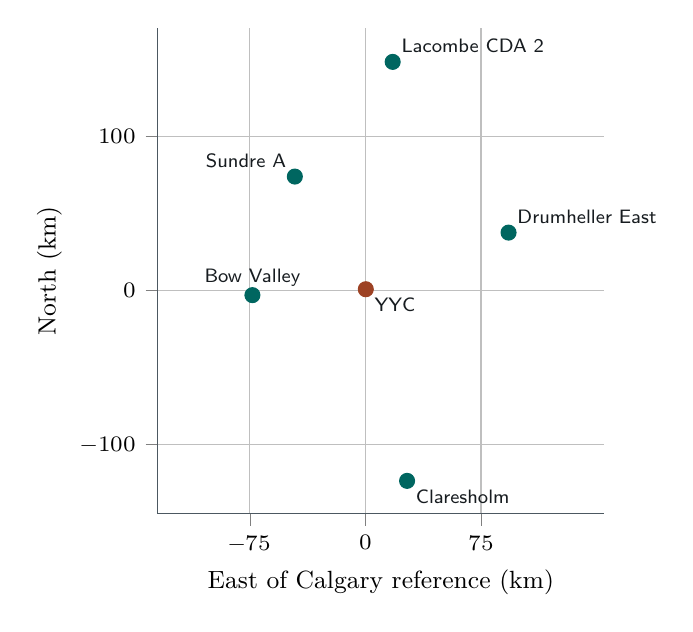
\begin{tikzpicture}\begin{axis}[weather,width=.83\linewidth,height=3.05in,axis equal image,xmin=-135,xmax=155,ymin=-145,ymax=170,xtick={-75,0,75},ytick={-100,0,100},xlabel={East of Calgary reference (km)},ylabel={North (km)},grid=major,clip=false]
\addplot[only marks,mark=*,mark size=2.7pt,color=rust] coordinates {(0.23,0.64)};
\node[font=\sffamily\scriptsize,inner sep=3pt,anchor=north west,text=ink] at (axis cs:0.23,0.64){YYC};
\addplot[only marks,mark=*,mark size=2.7pt,color=teal] coordinates {(-73.34,-3.19)};
\node[font=\sffamily\scriptsize,inner sep=3pt,anchor=south,text=ink] at (axis cs:-73.34,-3.19){Bow Valley};
\addplot[only marks,mark=*,mark size=2.7pt,color=teal] coordinates {(-45.81,73.75)};
\node[font=\sffamily\scriptsize,inner sep=3pt,anchor=south east,text=ink] at (axis cs:-45.81,73.75){Sundre A};
\addplot[only marks,mark=*,mark size=2.7pt,color=teal] coordinates {(92.86,37.38)};
\node[font=\sffamily\scriptsize,inner sep=3pt,anchor=south west,text=ink] at (axis cs:92.86,37.38){Drumheller East};
\addplot[only marks,mark=*,mark size=2.7pt,color=teal] coordinates {(27.02,-123.70)};
\node[font=\sffamily\scriptsize,inner sep=3pt,anchor=north west,text=ink] at (axis cs:27.02,-123.70){Claresholm};
\addplot[only marks,mark=*,mark size=2.7pt,color=teal] coordinates {(17.68,148.16)};
\node[font=\sffamily\scriptsize,inner sep=3pt,anchor=south west,text=ink] at (axis cs:17.68,148.16){Lacombe CDA 2};
\end{axis}\end{tikzpicture}
\caption{Hourly observing stations in southern Alberta. Distances are measured from the Calgary reference point.}\label{fig:network}
\end{figure}


Positions are calculated from the project inventory's great-circle distances and initial bearings relative to $51.1167^{\circ}$N, $114.0167^{\circ}$W. YYC lies approximately 0.7 km from that reference.

\paragraph{Record completeness and predictor choices.}
Table~\ref{tab:stations} reports completeness separately for temperature and pressure.



\begin{table}[!htbp]
\centering\small
\caption{Station identifiers, elevations and missing fractions for the 2016--2025 hourly record.}\label{tab:stations}
\renewcommand{\arraystretch}{1.08}\begin{tabular*}{.98\linewidth}{@{\extracolsep{\fill}}lrrrrr@{}}\toprule
\thead{Station} & \thead{ECCC ID} & \thead{Elev. (m)} & \thead{Distance (km)} & \thead{Temp. missing} & \thead{Pressure missing}\\\midrule
Calgary Intl A & 50430 & 1099 & 0.7 & 0.10\% & 0.10\% \\
Bow Valley & 10222 & 1298 & 73.4 & 0.81\% & 0.98\% \\
Sundre A & 10105 & 1114 & 86.8 & 1.56\% & 3.69\% \\
Drumheller East & 10708 & 678 & 100.1 & 1.96\% & 46.32\% \\
Claresholm & 2224 & 1009 & 126.6 & 0.38\% & 0.33\% \\
Lacombe CDA 2 & 10906 & 860 & 149.2 & 0.65\% & 25.82\% \\
\bottomrule\end{tabular*}
\end{table}


The five auxiliary sites span several directions and elevations. All provide temperature, dew point, relative humidity and wind speed. Pressure is also used at Bow Valley, Sundre and Claresholm. Pressure was missing for 46.3\% of the Drumheller record and 25.8\% at Lacombe. Station selection and pressure availability were assessed over the full study record. Model fitting used the earlier training years.


\subsection{Predictors, split dates and verification sample}\label{design}
At origin $t$ and lead $h\in\{1,6,12,24,48\}$ hours, a training case is $(x_t,T_{t+h})$. A row stores local observations, regional observations and the calendar at $t$. The verifying temperature $T_{t+h}$ is a separate column built by shifting YYC's regular hourly grid. The local and regional models are fitted independently at each lead.

Table~\ref{tab:features} defines the two nested sets of engineered predictors.



\begin{table}[!htbp]
\centering\small
\caption{Predictors available at a forecast origin. The first three groups constitute the airport-only input.}\label{tab:features}
\renewcommand{\arraystretch}{1.15}\begin{tabularx}{\linewidth}{@{}p{1.62in}rX@{}}\toprule\thead{Predictor group}&\thead{Count}&\thead{Values in the engineered vector}\\\midrule
Airport temperature & 24 & $T_t,T_{t-1},\ldots,T_{t-23}$, newest first, in \celsius.\\
Airport weather & 6 & Dew point (\celsius), humidity (\%), station pressure (kPa), wind speed (km/h), wind direction sine and cosine.\\
Calendar & 4 & Sine/cosine pairs for local hour and day of year.\\
Auxiliary observations & 33 & At each of five stations, temperature at $t,t-3,t-6$ and current dew point, humidity and wind speed. Three stations also contribute pressure.\\\bottomrule\end{tabularx}
\end{table}


The hour angle is $2\pi\,\mathrm{hour}(t)/24$ and the annual angle is $2\pi\,\mathrm{dayofyear}(t)/365.25$, with 1 January numbered 1. A reported wind direction in tens of degrees is multiplied by ten before taking the sine and cosine of its angle. These encodings keep times and directions on either side of a cycle boundary close together.

\paragraph{Eligibility and chronological splits.} Table~\ref{tab:cohort} traces the construction of the matched evaluation cohort.


\begin{table}[!htbp]
\centering\small
\caption{Successive restrictions defining the 2025 matched sample. Counts are distinct forecast origins.}\label{tab:cohort}
\renewcommand{\arraystretch}{1.08}\begin{tabular*}{.97\linewidth}{@{\extracolsep{\fill}}lr@{}}\toprule\thead{Cumulative condition on 2025 origins}&\thead{Hours remaining}\\\midrule
All hourly calendar slots & 8,760\\
The 48-hour verification also lies in 2025 & 8,712\\
Current YYC temperature and all five verifying temperatures observed & 8,664\\
Complete engineered airport inputs, allowing a zero direction vector for calm wind & 8,480\\
Reported local wind direction, as required in the matched regional experiment & 8,102\\\bottomrule\end{tabular*}
\end{table}


Auxiliary gaps remain eligible. At training and prediction time, a missing auxiliary value is replaced by that column's training median. The 378 hours in the final step had zero wind speed and a blank direction. This distinction explains why the original standalone airport experiment and the airport baseline inside the matched experiment have different scores.

Models trained on 2016--2023, selected settings or epochs in 2024 and were evaluated in 2025. A target had to remain in the same period as its origin. A forecast issued at 18:00 on 31 December 2023 with a six-hour lead therefore cannot be a training case. Screening for the availability of all five labels is a retrospective scoring choice. A new forecast from a manual vector requires no future observations.


\FloatBarrier
\section{Statistical methods}\label{methods}


\subsection{Nested information and reference forecasts}\label{information}
Let $Y=T_{t+h}$ and let $\mathcal F_t$ and $\mathcal G_t$ be the sigma-algebras generated by the airport and regional predictor vectors, respectively. Since the regional vector includes all airport predictors, $\mathcal F_t\subseteq\mathcal G_t$. The squared-error criterion yields the following projection identity.
\begin{proposition}\label{prop:information}
Suppose $Y\in L^2$. For $m_F=\mathbb E[Y\mid\mathcal F_t]$ and $m_G=\mathbb E[Y\mid\mathcal G_t]$,
\begin{equation}\label{eq:projection}
\mathbb E[(Y-m_F)^2]-\mathbb E[(Y-m_G)^2]=\mathbb E[(m_G-m_F)^2].
\end{equation}
\end{proposition}
\begin{proof}
Expand $Y-m_F=(Y-m_G)+(m_G-m_F)$. Since $m_G-m_F$ is $\mathcal G_t$-measurable, the cross term has expectation zero by conditioning on $\mathcal G_t$.
\end{proof}
Equation~\eqref{eq:projection} identifies the reduction in optimal population risk with the variability of the change in conditional mean. A trained network estimates each conditional mean with a finite function class and a finite record. For a fixed fitted predictor $f_G$ using regional information, the squared-error risk contains both the irreducible term $\mathbb E[(Y-m_G)^2]$ and the approximation and estimation term $\mathbb E[(f_G-m_G)^2]$. The empirical regional gain can therefore turn negative. The 48-hour reversal is consistent with several explanations, including estimation error, year-specific weather and a small incremental signal.

\paragraph{Reference forecasts.}
Persistence predicts the current reading, $\widehat T_{t+h}=T_t$. Two additional airport references use a table $c(m,k)$ of mean temperature at calendar month $m$ and local hour $k$. The table was estimated once on 70,055 finite training observations. Each of its 288 cells has 225--248 readings. Define $c(s)=c(\mathrm{month}(s),\mathrm{hour}(s))$. Then
\begin{equation}\label{eq:calendar}
 \widehat T^{\mathrm{calendar}}_{t+h}=c(t+h),\qquad
 \widehat T^{\mathrm{anomaly}}_{t+h}=c(t+h)+[T_t-c(t)].
\end{equation}
The anomaly forecast in \eqref{eq:calendar} carries today's departure from its typical temperature forward while allowing the usual daily heating or cooling. These are supplemental benchmarks specified in the retrospective analysis. They use the same 8,102 test origins and training years as the other comparisons, with no coefficients estimated on 2025.

At six hours, persistence scores 5.286\,\celsius{} and anomaly persistence 3.383\,\celsius. A substantial part of the error in carrying the raw reading forward is therefore avoidable with a calendar adjustment. The regional MLP still scores 2.328\,\celsius, about 31\% below the adjusted baseline. Table~\ref{tab:models} reports both benchmarks at every lead.


\subsection{Estimation and model selection}\label{estimators}
\paragraph{Preprocessing and ordinary least squares.}
For each lead, auxiliary medians, column means and standard deviations came from the eligible training rows. Missing values were filled before computing the means and standard deviations. A constant column received a scale of one. With standardized features $z_t$, ordinary least squares (OLS) fits an intercept and slopes by minimizing $\sum_t(Y_t-\beta_0-z_t^\top\beta)^2$. The local and regional fits use 34 and 67 predictors respectively. Since successive temperature lags are correlated, individual slope magnitudes alone give a poor guide to a station's incremental forecast value.

Principal-component regression (PCR) first diagonalizes the standardized training covariance and then fits OLS on the first $k$ score coordinates. At each lead, the validation set selected $k$ from $16,32,48,64$. All five fits selected 64, the upper end of the grid. At six hours the validation RMSE moved from 2.991 at 16 components to 2.698\,\celsius{} at 64. Discarding directions of small predictor variance can remove predictive information. The search gives no preference among the untested values 65--67.

\paragraph{Feed-forward neural networks.}
The primary matched MLP standardizes both the features and the training target. With one hidden ReLU layer, its raw-unit forecast is
\begin{equation}\label{eq:mlp}
 \widehat T_{t+h}=\bar Y_h+s_{Y,h}\left[b_2+w_2^\top\max\{0,W_1z_t+b_1\}\right].
\end{equation}
Both fits in \eqref{eq:mlp} have 32 hidden units. Increasing input width from 34 to 67 raises the parameter count from 1,153 to 2,209. Adam used learning rate $10^{-3}$, batch size 64 and weight decay $10^{-5}$. Each horizon and feature set kept its best validation checkpoint, with a cap of 200 epochs and patience of 15. This comparison measures adding features under a common fitting rule. It also changes the number of trainable weights.

The standalone airport search selected these settings in stages. Candidate learning rates were $10^{-4},3\times10^{-4},10^{-3}$, hidden widths were $(32),(64,32),(128,64)$, batch sizes were 64 and 256, and weight decay was $0,10^{-5},10^{-4}$. The criterion was $Q=\frac15\sum_h R_{\text{MLP},h}^{\rm val}/R_{\text{OLS},h}^{\rm val}$. Ratios give each lead comparable influence despite the larger errors at long leads. The selected configuration scored $Q=0.9178$. The matched comparison reused its settings and fitted a separate model pair on the shared cohort.

\paragraph{Boosted decision trees.}
LightGBM~\cite{lightgbm} used the 67 engineered features with training-median imputation. Each lead allowed 500 trees, learning rate 0.04, up to 31 leaves, at least 30 observations per leaf and 80\% feature sampling per tree. Validation early stopping had patience 40. Selected iterations were 498, 500, 482, 190 and 154 in increasing lead order. The six-hour fit reached the search ceiling.


\subsection{Joint sequence models}\label{sequence}
Hourly trajectories can be given directly to a model. A separate experiment uses four readings at each of six stations (temperature, dew point, relative humidity and wind speed) for each of the 24 hours ending at the origin. Every value channel has a paired indicator equal to one when observed. Values are median-imputed and standardized with training-period statistics before appending the masks. The result has 24 time steps and 48 channels. The four cyclic calendar features accompany the sequence.

Both sequence models jointly forecast the same five temperatures, each standardized using its training target distribution. A common train/validation/test rule keeps the 48-hour target in its split, yielding 69,630, 8,682 and 8,664 origins respectively. The published architecture comparison reindexes the sequence predictions to the 8,102 engineered-model origins.

\paragraph{Two ways of processing the same history.}
The sequence MLP flattens the $24\times48$ tensor and appends the four calendar coordinates. Its hidden widths are 128 and 64, with GELU activations and dropout 0.10. The compact temporal convolutional network (TCN) projects the 48 channels to 16 and applies four causal residual blocks. A width-three kernel with dilation $d$ uses positions $t,t-d,t-2d$. With dilations $1,2,4,8$, the receptive field is $1+2(1+2+4+8)=31$ time steps. Left padding allows the final output to depend on the whole 24-hour input. The final time step and calendar enter a dense output head~\cite{tcn}.

The sequence models used AdamW, a learning rate of $8\times10^{-4}$, weight decay $10^{-5}$, batches of 4,096 origins and patience three. Each of the six runs selected epoch 15, the cap. The MLP has 156,677 parameters and the compact TCN 4,757. The fixed computational budget and unequal capacities matter when interpreting an architecture ranking.


\subsection{Forecast verification and paired inference}\label{uncertainty}
For a common set $\mathcal I_h$ of $n_h$ origins, let $e_{m,t,h}=\widehat T^{(m)}_{t+h}-T_{t+h}$. Positive bias denotes a warm forecast. We evaluate error magnitude, signed bias, and squared error through
\begin{equation}\label{eq:errors}
 \mathrm{MAE}_{m,h}=\frac1{n_h}\sum_{t\in\mathcal I_h}|e_{m,t,h}|,\quad
 B_{m,h}=\frac1{n_h}\sum_{t\in\mathcal I_h}e_{m,t,h},\quad
 R_{m,h}=\left(\frac1{n_h}\sum_{t\in\mathcal I_h}e_{m,t,h}^2\right)^{1/2}.
\end{equation}
With $A$ denoting the airport fit and $S$ the regional fit, the absolute and relative RMSE improvements are
\begin{equation}\label{eq:gain}
 D_h=R_{A,h}-R_{S,h},\qquad G_h=100\left(1-\frac{R_{S,h}}{R_{A,h}}\right).
\end{equation}
The units of $D_h$ are \celsius{}, and $G_h$ is a percentage relative to the airport model. Specifying the reference and the scoring scale is essential when interpreting a skill score~\cite{murphy}.
The percentage depends on the scoring scale. At six hours, $G=13.02\%$, while the reduction in mean \emph{squared} error is $100[1-(R_S/R_A)^2]=24.35\%$. The absolute MSE difference is 1.744\,\celsius$^2$. A statement about the percentage reduction in temperature forecast error should specify RMSE to avoid conflating these quantities.

\paragraph{A paired calendar-day block bootstrap.}
Consecutive forecasts share inputs and experience related weather. We aggregated the two squared-error sums and the number of valid pairs for every origin date in 2025. A draw samples starting dates uniformly with replacement and takes $L$ consecutive calendar days from each start, wrapping at year end. Blocks are concatenated and the last one is truncated at 365 days. Both forecasts, all leads and the counts move together. A date with no eligible hours contributes zero error and zero observations~\cite{politis}.

Each draw recomputes both RMSEs from its resampled sums and counts, then recomputes the percentage ratio. The reported bounds are the 2.5th and 97.5th percentiles of 5,000 draws, seed 2403. Aggregating only the paired loss differences would suffice for an MSE difference, but the nonlinear RMSE ratio requires both squared-error sums.


For a bootstrap draw, let $w_d$ count the occurrences of calendar day $d$, let $n_{d,h}$ count valid origins on that day, and set $S_{d,m,h}=\sum_{t\in d\cap\mathcal I_h}e_{m,t,h}^2$. The resampled estimate in \eqref{eq:errors} is
\begin{equation}\label{eq:resample}
 R^*_{m,h}=\left(\frac{\sum_d w_d S_{d,m,h}}{\sum_d w_d n_{d,h}}\right)^{1/2}.
\end{equation}
Using the same $w_d$ in both models in \eqref{eq:gain} preserves the paired losses. Equation~\eqref{eq:resample} also gives days with more eligible forecasts their appropriate weight.


\FloatBarrier
\section{Results}\label{results}


\subsection{Incremental regional skill and sensitivity to case selection}\label{matched}
The primary comparison holds the forecast origin, verifying observation, lead and fitting procedure fixed. At six hours, adding the regional predictors saved 0.349\,\celsius{} in RMSE. The same change lowered mean absolute error from 1.945 to 1.724\,\celsius. The agreement of the two measures shows that the improvement extends beyond the greater weight that RMSE assigns to large errors.

Table~\ref{tab:main} reports the primary estimates. Table~\ref{tab:selection} gives the corresponding training counts, selected epochs and validation gains.



\begin{table}[!htbp]
\centering\small
\caption{Matched test-year RMSE (\celsius) and percentage reduction from regional observations. The seven-day interval is pointwise.}\label{tab:main}
\renewcommand{\arraystretch}{1.12}\begin{tabular*}{.97\linewidth}{@{\extracolsep{\fill}}lrrrr@{}}\toprule
\thead{Lead} & \thead{Airport MLP} & \thead{Six-station MLP} & \thead{RMSE reduction} & \thead{95\% block interval}\\\midrule
1 h & 1.073 & 0.986 & 8.15\% & [6.77, 9.70] \\
6 h & 2.676 & 2.328 & 13.02\% & [10.29, 15.78] \\
12 h & 3.551 & 3.244 & 8.65\% & [5.97, 11.37] \\
24 h & 4.634 & 4.457 & 3.82\% & [1.77, 5.57] \\
48 h & 5.750 & 5.782 & −0.55\% & [−2.85, 1.47] \\
\bottomrule\end{tabular*}
\end{table}





\begin{table}[!htbp]
\centering\small
\caption{Training and validation cases, selected epochs, and regional gains by lead.}\label{tab:selection}
\renewcommand{\arraystretch}{1.14}\begin{tabular*}{.99\linewidth}{@{\extracolsep{\fill}}lrrrrrr@{}}\toprule
 & \multicolumn{2}{c}{\thead{Eligible origins}} & \multicolumn{2}{c}{\thead{Best epoch}} & \multicolumn{2}{c}{\thead{Regional RMSE reduction}}\\
\cmidrule(lr){2-3}\cmidrule(lr){4-5}\cmidrule(l){6-7}\thead{Lead}&\thead{Train}&\thead{Validation}&\thead{Airport}&\thead{Regional}&\thead{2024 validation}&\thead{2025 test}\\\midrule
1 h & 65,443 & 8,209 & 57 & 109 & 7.13\% & 8.15\% \\
6 h & 65,438 & 8,204 & 61 & 35 & 10.72\% & 13.02\% \\
12 h & 65,432 & 8,198 & 49 & 43 & 7.20\% & 8.65\% \\
24 h & 65,421 & 8,187 & 24 & 11 & 4.93\% & 3.82\% \\
48 h & 65,397 & 8,164 & 14 & 19 & 2.83\% & −0.55\% \\
\bottomrule\end{tabular*}
\end{table}


The direction of the six-hour result repeats across the two years, with validation RMSE falling from 2.473 to 2.208\,\celsius. The 48-hour validation result favoured the regional model, while the test result favoured the airport model. Validation informed checkpoint selection, so the two years have different evidential roles. Their disagreement at 48 hours makes a general two-day gain difficult to support.

\paragraph{Sensitivity to calm-wind eligibility.}
For each of 378 additional origins, the local wind speed was zero and direction was missing. Encoding the direction pair as $(0,0)$ supplies a distinct calm state. The fitted matched networks and their original training scalers were applied to these extra cases. This checks the effect of the test case definition. It does not measure how a new fit trained with calm origins would behave.

Table~\ref{tab:calm} shows the sensitivity of $G_h$ to eligibility.



\begin{table}[!htbp]
\centering\small
\caption{Relative RMSE reduction under alternative treatment of calm-wind origins.}\label{tab:calm}
\renewcommand{\arraystretch}{1.12}\begin{tabular*}{.95\linewidth}{@{\extracolsep{\fill}}lrrr@{}}\toprule\thead{Lead}&\thead{8,102 original hours}&\thead{378 additional calm hours}&\thead{8,480 combined hours}\\\midrule
1 h & 8.15\% & 7.06\% & 8.08\% \\
6 h & 13.02\% & 20.53\% & 13.43\% \\
12 h & 8.65\% & 14.25\% & 8.94\% \\
24 h & 3.82\% & 0.98\% & 3.71\% \\
48 h & −0.55\% & −0.49\% & −0.55\% \\
\bottomrule\end{tabular*}
\end{table}


Entries are relative reductions in RMSE from the airport MLP to the six-station MLP. Each column uses the same fitted pair. The combined percentage is computed after pooling squared errors.

At six hours the expanded sample yielded 2.693 versus 2.331\,\celsius{}, a 13.43\% reduction. At 48 hours the combined reduction was $-0.55\%$. The project also contains a separately trained \code{standalone-local} network. Substituting its RMSE into the primary ratio would change both the fitted baseline and its evaluation cohort.


Table~\ref{tab:blocks} compares intervals based on three choices of block length.



\begin{table}[!htbp]
\centering\small
\caption{Pointwise 95\% intervals for the relative RMSE reduction (percent), by calendar block length.}\label{tab:blocks}
\renewcommand{\arraystretch}{1.14}\begin{tabular*}{.95\linewidth}{@{\extracolsep{\fill}}lrrr@{}}\toprule\thead{Lead}&\thead{3-day blocks}&\thead{7-day blocks}&\thead{14-day blocks}\\\midrule
1 h & [6.72, 9.73] & [6.77, 9.70] & [6.79, 9.62] \\
6 h & [10.53, 15.34] & [10.29, 15.78] & [9.78, 15.99] \\
12 h & [6.10, 11.19] & [5.97, 11.37] & [5.81, 11.35] \\
24 h & [1.78, 5.78] & [1.77, 5.57] & [1.69, 5.49] \\
48 h & [−2.81, 1.73] & [−2.85, 1.47] & [−2.97, 1.48] \\
\bottomrule\end{tabular*}
\end{table}



Pointwise 95\% intervals for regional RMSE reduction, in percent. They condition on the fitted networks and the weather sampled in the 2025 archive.

Changing block length leaves the first four lead-specific intervals above zero and the 48-hour intervals spanning zero. Year-to-year shifts, retraining variability, the choice of target airport and simultaneous error control across all five leads lie outside these bounds. Resampling blocks of a single seasonal record also moves the proportion of winter and summer dates from draw to draw.


\subsection{Model comparisons on common forecast origins}\label{comparison}
All entries below use 8,102 observations per lead. PCR was refitted on the same design, with component count chosen on 2024. The two calendar references use training-only airport readings. Sequence entries average the RMSEs of three individual fits after aligning their origins and verifying observations.

Table~\ref{tab:models} places the matched comparisons on the same RMSE scale.



\begin{table}[!htbp]
\centering\small
\caption{Test-year RMSE by forecast method and lead, in \celsius. Bold entries are column minima.}\label{tab:models}
\renewcommand{\arraystretch}{1.12}\begin{tabular*}{.98\linewidth}{@{\extracolsep{\fill}}lrrrrr@{}}\toprule\thead{2025 RMSE (\celsius)}&\thead{1 h}&\thead{6 h}&\thead{12 h}&\thead{24 h}&\thead{48 h}\\\midrule
Persistence & 1.411 & 5.286 & 7.264 & 5.770 & 7.216 \\
Month/hour climatology & 6.748 & 6.724 & 6.692 & 6.696 & 6.692 \\
Anomaly persistence & 1.168 & 3.383 & 4.684 & 5.853 & 7.327 \\
Airport OLS & 1.158 & 3.156 & 4.037 & 4.858 & 5.854 \\
Regional OLS & 1.084 & 2.844 & 3.707 & 4.652 & 5.790 \\
Regional PCR & 1.122 & 2.845 & 3.710 & 4.648 & 5.787 \\
Airport MLP & 1.073 & 2.676 & 3.551 & 4.634 & 5.750 \\
Regional MLP & \bestscore{0.986} & \bestscore{2.328} & \bestscore{3.244} & 4.457 & 5.782 \\
Regional LightGBM & 1.027 & 2.461 & 3.334 & \bestscore{4.455} & \bestscore{5.695} \\
Sequence MLP (mean) & 1.683 & 2.858 & 3.751 & 4.814 & 6.084 \\
Sequence TCN (mean) & 2.033 & 3.160 & 3.988 & 4.973 & 6.138 \\
\bottomrule\end{tabular*}
\end{table}


At six hours, the airport MLP improves on airport OLS by 0.480\,\celsius. Adding regional predictors to OLS improves it by 0.312\,\celsius, and a six-station MLP improves on that regional OLS fit by a further 0.516\,\celsius. The observations help a linear model as well as a nonlinear model. The size of either contribution depends on the reference in the comparison.

\paragraph{Pairwise comparison with boosted trees.}
With the same features, the MLP has the lowest measured RMSE through 12 hours, while LightGBM has the lowest observed values at 24 and 48 hours. The latter two rankings rest on small gaps. For a paired check, the reference here is the regional MLP and the candidate is LightGBM. Positive differences favour the tree model.

Table~\ref{tab:tree} quantifies the uncertainty in these pairwise rankings.



\begin{table}[!htbp]
\centering\small
\caption{Regional MLP minus LightGBM RMSE, with paired seven-day block intervals, in \celsius. Positive values favour LightGBM.}\label{tab:tree}
\renewcommand{\arraystretch}{1.08}\begin{tabular*}{.93\linewidth}{@{\extracolsep{\fill}}lrr@{}}\toprule\thead{Lead}&\thead{MLP RMSE minus LightGBM RMSE}&\thead{95\% block interval (\celsius)}\\\midrule
1 h & −0.041 & [−0.056, −0.028] \\
6 h & −0.133 & [−0.194, −0.069] \\
12 h & −0.089 & [−0.197, 0.032] \\
24 h & +0.002 & [−0.089, 0.104] \\
48 h & +0.087 & [−0.060, 0.239] \\
\bottomrule\end{tabular*}
\end{table}


The within-year intervals put the regional MLP ahead at one and six hours. The 12-hour point estimate also favours it, with an interval spanning zero. LightGBM's 48-hour lead of 0.087\,\celsius{} has an interval from $-0.060$ to $+0.239$\,\celsius. A firm ranking of the two methods at two days would need additional independent forecast periods.


\paragraph{Variation across sequence fits.} Table~\ref{tab:sequence} shows the across-seed spread for the two joint models.



\begin{table}[!htbp]
\centering\small
\caption{Matched forecast RMSE by architecture. Entries give the mean and sample standard deviation across three fitted seeds, in \celsius.}\label{tab:sequence}
\renewcommand{\arraystretch}{1.12}\begin{tabular*}{.97\linewidth}{@{\extracolsep{\fill}}lrrrrr@{}}\toprule\thead{Matched RMSE (\celsius)} & \thead{1 h} & \thead{6 h} & \thead{12 h} & \thead{24 h} & \thead{48 h}\\\midrule
Sequence MLP & 1.68 $\pm$ 0.06 & 2.86 $\pm$ 0.01 & 3.75 $\pm$ 0.02 & 4.81 $\pm$ 0.04 & 6.08 $\pm$ 0.03 \\
Sequence TCN & 2.03 $\pm$ 0.03 & 3.16 $\pm$ 0.03 & 3.99 $\pm$ 0.01 & 4.97 $\pm$ 0.03 & 6.14 $\pm$ 0.03 \\
\bottomrule\end{tabular*}
\end{table}



Entries give mean RMSE and sample standard deviation over seeds 17, 2026 and 2403. Each seed's predictions are scored separately. Averaging forecasts across seeds would define a different model.

The flattened MLP had lower mean RMSE at all five leads within this shared-input comparison. Relative to the engineered MLP, both sequence systems also change the predictor variables, training cohort, parameter count and multi-output loss. Their performance cannot isolate the effect of replacing engineered features with raw histories.


\subsection{Station ablation and the Bow Valley temperature contrast}\label{ablation}
For each lead, a regional OLS model was fitted with one auxiliary station's entire group of predictors removed. The remaining columns, airport features, training dates and test cases stayed fixed. Each entry in Table~\ref{tab:ablation} is the reduced model's test RMSE minus full-model RMSE. Positive values show the error incurred by removing that station, conditional on all the other sites.



\begin{table}[!htbp]
\centering\small
\caption{Change in OLS test RMSE after omitting each group of regional observations, in \celsius. Positive values denote higher error after removal.}\label{tab:ablation}
\renewcommand{\arraystretch}{1.10}\begin{tabular*}{.96\linewidth}{@{\extracolsep{\fill}}lrrrrr@{}}\toprule\thead{Omitted observations}&\thead{1 h}&\thead{6 h}&\thead{12 h}&\thead{24 h}&\thead{48 h}\\\midrule
Bow Valley & 0.015 & 0.148 & 0.161 & 0.127 & 0.062 \\
Sundre A & 0.022 & 0.057 & 0.071 & 0.025 & 0.009 \\
Drumheller East & −0.002 & 0.003 & 0.018 & 0.002 & −0.005 \\
Claresholm & 0.005 & 0.016 & 0.018 & −0.005 & −0.004 \\
Lacombe CDA 2 & 0.005 & 0.036 & 0.030 & 0.024 & 0.000 \\
All regional non-temperature variables & 0.023 & 0.180 & 0.216 & 0.073 & 0.039 \\
All five auxiliary stations & 0.074 & 0.312 & 0.330 & 0.206 & 0.064 \\
\bottomrule\end{tabular*}
\end{table}


Bow Valley produced the largest removal penalty at 6, 12 and 24 hours. At one hour, Sundre's penalty was larger. At six hours, using all regional temperature lags alongside the airport features but dropping the other regional variables raised error by 0.180\,\celsius{} relative to the full fit. Temperature alone retained some of the improvement. The station removal penalties need not sum to the all-stations penalty because neighbouring predictors can carry overlapping information.

\paragraph{A temperature contrast observable at issue time.}
The Bow Valley result motivates a second question. Is the six-hour MLP gain concentrated on hours with a large temperature contrast between Bow Valley and YYC? We grouped origins by $|T_{\rm Bow}(t)-T_{\rm YYC}(t)|$. The cut points 1.0, 2.1 and 3.8\,\celsius{} are training quartiles from 64,821 six-hour training cases with both readings available. Boundaries include their upper endpoint. Ties explain the unequal 2025 group sizes.

Table~\ref{tab:contrast} reports the resulting groups and their paired scores.



\begin{table}[!htbp]
\centering\small
\caption{Six-hour test errors by absolute Bow Valley--YYC temperature contrast at issuance. RMSE is in \celsius.}\label{tab:contrast}
\renewcommand{\arraystretch}{1.10}\begin{tabular*}{.96\linewidth}{@{\extracolsep{\fill}}lrrrr@{}}\toprule\thead{Origin contrast (\celsius)}&\thead{Cases}&\thead{Airport RMSE}&\thead{Regional RMSE}&\thead{Gain}\\\midrule
$[0,1.0]$ & 2,169 & 2.480 & 2.145 & 13.53\% \\
$(1.0,2.1]$ & 2,006 & 2.603 & 2.253 & 13.45\% \\
$(2.1,3.8]$ & 1,985 & 2.769 & 2.355 & 14.93\% \\
$>3.8$ & 1,928 & 2.867 & 2.549 & 11.08\% \\
\bottomrule\end{tabular*}
\end{table}


Regional gains appear in all four observed-contrast groups, with the highest percentage in the third group. The quartile results give little support to a rule that adds regional inputs only at the largest gradients. The 14 origins with a missing current Bow Valley temperature are reported separately in the project tables. Their small count and possible clustering make an outage-specific skill estimate unstable. Neither this stratification nor the OLS ablation directly measures advection, wind direction or a causal effect.


\subsection{Seasonal heterogeneity}\label{seasons}
Seasons use the month of the \emph{verifying} observation. Winter (DJF) combines January, February and December of the 2025 test year. A forecast issued just before a season boundary can therefore enter a different group at a longer lead. The analysis compares identical local and regional forecast cases within each group.

Figure~\ref{fig:season} shows absolute errors, while Table~\ref{tab:seasons} gives their reduction relative to the airport-only fit.



\begin{figure}[!htbp]
\centering
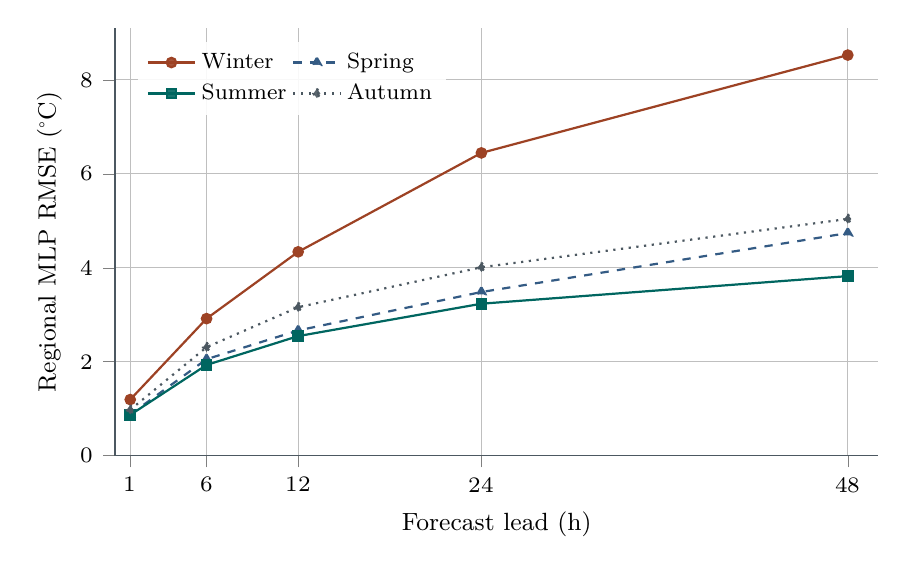
\begin{tikzpicture}\begin{axis}[weather,height=2.76in,xmin=0,xmax=50,ymin=0,ymax=9.1,xtick={1,6,12,24,48},ytick={0,2,4,6,8},xlabel={Forecast lead (h)},ylabel={Regional MLP RMSE (\celsius)},ymajorgrids,legend pos=north west,legend columns=2]
\addplot[rust,mark=*,thick,mark size=1.7pt] coordinates {(1,1.1945) (6,2.9178) (12,4.3398) (24,6.4454) (48,8.5283)};
\addlegendentry{Winter}
\addplot[blue,mark=triangle*,dashed,thick,mark size=1.7pt] coordinates {(1,0.8762) (6,2.0540) (12,2.6663) (24,3.4841) (48,4.7391)};
\addlegendentry{Spring}
\addplot[teal,mark=square*,thick,mark size=1.7pt] coordinates {(1,0.8679) (6,1.9317) (12,2.5458) (24,3.2351) (48,3.8229)};
\addlegendentry{Summer}
\addplot[slate,mark=diamond*,dotted,thick,mark size=1.7pt] coordinates {(1,0.9783) (6,2.3094) (12,3.1607) (24,4.0108) (48,5.0396)};
\addlegendentry{Autumn}
\end{axis}\end{tikzpicture}
\caption{Regional MLP test-year RMSE by season of the verifying observation. Lines join the five fitted leads.}\label{fig:season}
\end{figure}


\paragraph{Relative gain from the five auxiliary stations.}


\begin{table}[!htbp]
\centering\small
\caption{Percentage RMSE reduction from adding regional observations, by season of verification.}\label{tab:seasons}
\renewcommand{\arraystretch}{1.12}\begin{tabular*}{.94\linewidth}{@{\extracolsep{\fill}}lrrrrr@{}}\toprule\thead{Valid-time season}&\thead{1 h}&\thead{6 h}&\thead{12 h}&\thead{24 h}&\thead{48 h}\\\midrule
Winter (DJF) & 8.79\% & 16.07\% & 10.03\% & 5.83\% & 1.96\% \\
Spring (MAM) & 10.03\% & 12.67\% & 7.47\% & 2.50\% & −2.02\% \\
Summer (JJA) & 6.89\% & 9.33\% & 8.36\% & −0.25\% & −3.36\% \\
Autumn (SON) & 6.60\% & 10.69\% & 6.99\% & 2.07\% & −5.35\% \\
\bottomrule\end{tabular*}
\end{table}


At six hours the regional MLP improved RMSE in every season, from 9.33\% in summer to 16.07\% in winter. Winter supplied 1,981 of 8,102 six-hour cases, around one quarter. It supplied \textbf{50.1\% of the total reduction in squared error}. For that calculation the numerator is the winter sum of $e_A^2-e_S^2$, and the denominator is the same sum across the year. Difficult cases give a larger contribution to an annual RMSE calculation.

At 48 hours, winter still favoured the regional network by 1.96\%, while all three other seasonal point estimates favoured the airport network. The winter regional RMSE of 8.53\,\celsius{} was more than twice the summer value of 3.82\,\celsius. Winter contributed 53.1\% of annual regional squared error at that lead. These patterns describe the sampled months in 2025. Several winters would be needed to establish whether this concentration recurs.


\subsection{Large errors and conditional bias}\label{tails}
RMSE emphasizes large errors. A complementary question is how often a forecast improves and how far the upper tail of absolute error extends. In Table~\ref{tab:tails}, $q_{.95}$ is the empirical 95th percentile of absolute error. ``Closer'' counts a strict improvement by the regional MLP on an individual pair.



\begin{table}[!htbp]
\centering\small
\caption{Upper-tail absolute errors and the fraction of origins on which the regional MLP was closer.}\label{tab:tails}
\renewcommand{\arraystretch}{1.13}\begin{tabular*}{.98\linewidth}{@{\extracolsep{\fill}}lrrrrr@{}}\toprule
 & \multicolumn{2}{c}{\thead{$q_{.95}$ of $|e|$ (\celsius)}} & \multicolumn{2}{c}{\thead{Frequency $|e|\ge5\,\celsius$}} & \thead{Regional}\\
\cmidrule(lr){2-3}\cmidrule(lr){4-5}\thead{Lead}&\thead{Airport}&\thead{Regional}&\thead{Airport}&\thead{Regional}&\thead{closer}\\\midrule
1 h & 2.063 & 1.984 & 0.43\% & 0.30\% & 53.52\% \\
6 h & 5.389 & 4.734 & 6.12\% & 4.02\% & 56.34\% \\
12 h & 7.261 & 6.527 & 13.03\% & 11.10\% & 54.17\% \\
24 h & 9.176 & 8.957 & 23.33\% & 22.17\% & 52.46\% \\
48 h & 11.895 & 11.866 & 33.50\% & 34.52\% & 47.72\% \\
\bottomrule\end{tabular*}
\end{table}


At six hours the median absolute error fell from 1.445 to 1.310\,\celsius{} and the 95th percentile from 5.389 to 4.734\,\celsius. The regional model won on just over half the individual hours. The improvement in the size and frequency of larger misses helps explain how that modest fraction of wins produced a 13.02\% RMSE gain. At 48 hours the local model was closer more often, and the two 95th percentiles were nearly equal.

\paragraph{Bias conditional on verifying temperature.}
At six hours the regional annual mean error was $-0.070$\,\celsius, and at 48 hours it was $-0.043$\,\celsius. Grouping by the verifying temperature reveals errors that cancel in the annual mean. Table~\ref{tab:bands} uses lower-inclusive, upper-exclusive temperature bands.



\begin{table}[!htbp]
\centering\small
\caption{Regional MLP bias and RMSE in \celsius{} by observed temperature at verification. Bias is forecast minus observed.}\label{tab:bands}
\renewcommand{\arraystretch}{1.12}\begin{tabular*}{.97\linewidth}{@{\extracolsep{\fill}}lrrrrrr@{}}\toprule
 & \multicolumn{3}{c}{\thead{6 h regional MLP}}&\multicolumn{3}{c}{\thead{48 h regional MLP}}\\
\cmidrule(lr){2-4}\cmidrule(l){5-7}\thead{Verifying temp. (\celsius)}&\thead{Cases}&\thead{Bias}&\thead{RMSE}&\thead{Cases}&\thead{Bias}&\thead{RMSE}\\\midrule
$T < -10$ & 1,024 & +0.69 & 2.77 & 981 & +7.02 & 9.07 \\
$[-10,0)$ & 1,209 & +0.64 & 2.39 & 1,235 & +1.47 & 5.01 \\
$[0,10)$ & 2,401 & −0.09 & 2.41 & 2,397 & −1.62 & 5.93 \\
$[10,20)$ & 2,662 & −0.43 & 2.06 & 2,642 & −0.84 & 4.53 \\
$T \ge 20$ & 806 & −0.84 & 2.20 & 847 & −3.45 & 4.93 \\
\bottomrule\end{tabular*}
\end{table}


For verifying temperatures below $-10$\,\celsius{}, the two-day regional forecast was on average 7.02\,\celsius{} too warm. For temperatures of at least 20\,\celsius{}, it was 3.45\,\celsius{} too cool. These groups use an outcome unknown at issuance. Even an ideal conditional-mean forecast $m(X)$ has $\operatorname{Cov}(m(X)-Y,Y)=-\mathbb E[\operatorname{Var}(Y\mid X)]$. This follows by writing $Y=m(X)+[Y-m(X)]$ and using orthogonality. Grouping on the outcome can therefore reveal a tendency towards the centre even when the predictor is calibrated conditional on its inputs. A correction intended for live use would need a diagnostic based on information available at the origin.


\subsection{Two illustrative forecast periods}\label{cases}
Figure~\ref{fig:weeks} shows the first seven calendar days of February and July, chosen by calendar to give winter and summer examples. Each forecast is plotted at its \emph{valid} time, six hours after its origin. Breaks in a forecast line mark hours outside the matched evaluation set. The observed line uses the hourly airport record.



\begin{figure}[!htbp]
\centering
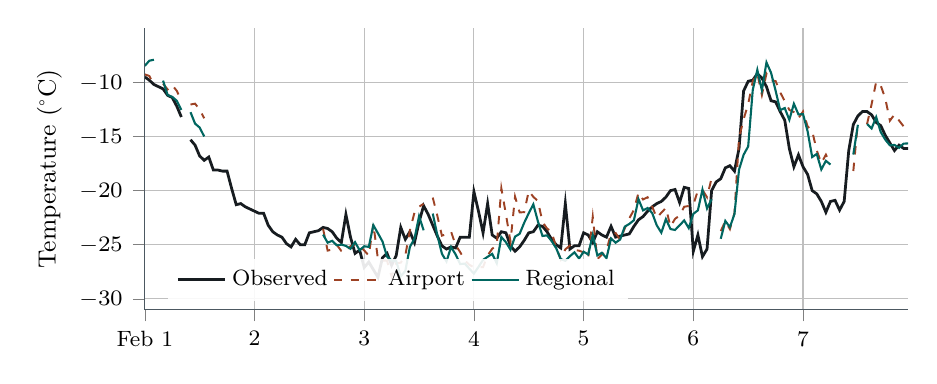
\begin{tikzpicture}\begin{axis}[weather,height=2.03in,xmin=0,xmax=167,ymin=-31,ymax=-5,xtick={0,24,48,72,96,120,144},xticklabels={Feb 1,2,3,4,5,6,7},ytick={-30,-25,-20,-15,-10},ylabel={Temperature (\celsius)},ymajorgrids,unbounded coords=jump,legend pos=south west,legend columns=3]
\addplot[ink,line width=1.0pt] coordinates {(0,-9.5000) (1,-9.8000) (2,-10.2000) (3,-10.4000) (4,-10.6000) (5,-11.2000) (6,-11.4000) (7,-12.2000) (8,-13.2000) (9,nan) (10,-15.3000) (11,-15.8000) (12,-16.8000) (13,-17.2000) (14,-16.9000) (15,-18.1000) (16,-18.1000) (17,-18.2000) (18,-18.2000) (19,-19.8000) (20,-21.3000) (21,-21.2000) (22,-21.5000) (23,-21.7000) (24,-21.9000) (25,-22.1000) (26,-22.1000) (27,-23.2000) (28,-23.8000) (29,-24.1000) (30,-24.3000) (31,-24.9000) (32,-25.2000) (33,-24.5000) (34,-25.0000) (35,-25.0000) (36,-23.9000) (37,-23.8000) (38,-23.7000) (39,-23.4000) (40,-23.5000) (41,-23.8000) (42,-24.4000) (43,-24.8000) (44,-22.2000) (45,-24.3000) (46,-25.8000) (47,-25.5000) (48,-27.1000) (49,-26.6000) (50,-27.3000) (51,-28.0000) (52,-26.2000) (53,-25.8000) (54,-26.9000) (55,-26.0000) (56,-23.4000) (57,-24.5000) (58,-23.8000) (59,-24.8000) (60,-22.9000) (61,-21.4000) (62,-22.2000) (63,-23.2000) (64,-24.2000) (65,-25.1000) (66,-25.4000) (67,-25.2000) (68,-25.3000) (69,-24.3000) (70,-24.3000) (71,-24.3000) (72,-20.1000) (73,-21.9000) (74,-23.9000) (75,-21.2000) (76,-24.1000) (77,-24.4000) (78,-23.8000) (79,-23.9000) (80,-25.1000) (81,-25.6000) (82,-25.2000) (83,-24.6000) (84,-23.9000) (85,-23.8000) (86,-23.2000) (87,-23.3000) (88,-23.8000) (89,-24.5000) (90,-25.0000) (91,-25.3000) (92,-21.2000) (93,-25.4000) (94,-25.1000) (95,-25.1000) (96,-23.9000) (97,-24.1000) (98,-24.8000) (99,-23.8000) (100,-24.1000) (101,-24.3000) (102,-23.3000) (103,-24.3000) (104,-24.2000) (105,-24.1000) (106,-24.0000) (107,-23.3000) (108,-22.7000) (109,-22.4000) (110,-21.9000) (111,-21.5000) (112,-21.2000) (113,-21.0000) (114,-20.6000) (115,-20.0000) (116,-19.9000) (117,-21.1000) (118,-19.7000) (119,-19.8000) (120,-25.6000) (121,-24.1000) (122,-26.1000) (123,-25.4000) (124,-20.0000) (125,-19.2000) (126,-18.9000) (127,-17.9000) (128,-17.7000) (129,-18.2000) (130,-16.1000) (131,-10.8000) (132,-9.9000) (133,-9.8000) (134,-9.2000) (135,-9.6000) (136,-10.4000) (137,-11.7000) (138,-11.8000) (139,-12.7000) (140,-13.5000) (141,-16.1000) (142,-17.8000) (143,-16.7000) (144,-17.8000) (145,-18.5000) (146,-20.0000) (147,-20.3000) (148,-21.0000) (149,-22.0000) (150,-21.0000) (151,-20.9000) (152,-21.8000) (153,-21.0000) (154,-16.3000) (155,-13.9000) (156,-13.1000) (157,-12.7000) (158,-12.7000) (159,-13.0000) (160,-13.7000) (161,-14.0000) (162,-14.9000) (163,-15.6000) (164,-16.3000) (165,-15.8000) (166,-16.1000) (167,-16.1000)};
\addlegendentry{Observed}
\addplot[rust,dashed,line width=0.70pt] coordinates {(0,-9.2666) (1,-9.4113) (2,-10.2542) (3,nan) (4,-10.1319) (5,-10.6565) (6,-10.2557) (7,-10.7853) (8,-11.6861) (9,nan) (10,-12.0453) (11,-11.9692) (12,-12.5082) (13,-13.3183) (14,nan) (15,nan) (16,nan) (17,nan) (18,nan) (19,nan) (20,nan) (21,nan) (22,nan) (23,nan) (24,nan) (25,nan) (26,nan) (27,nan) (28,nan) (29,nan) (30,nan) (31,nan) (32,nan) (33,nan) (34,nan) (35,nan) (36,nan) (37,nan) (38,nan) (39,-23.5273) (40,-25.5419) (41,-25.4435) (42,-25.0077) (43,-25.5792) (44,-25.6700) (45,-25.1285) (46,-24.9859) (47,-25.1112) (48,-25.5243) (49,-26.0052) (50,-23.0646) (51,-26.3246) (52,-26.4626) (53,-26.4870) (54,-27.9561) (55,-26.7136) (56,-26.6598) (57,-25.9652) (58,-23.6625) (59,-22.0303) (60,-21.4883) (61,-21.2204) (62,nan) (63,-20.6456) (64,-22.3312) (65,-24.1591) (66,-24.0315) (67,-23.7865) (68,-25.0533) (69,-25.6811) (70,-26.4560) (71,-26.8539) (72,-27.0798) (73,-27.0622) (74,-27.0695) (75,-25.9860) (76,-25.3782) (77,-25.0422) (78,-19.7775) (79,-22.1776) (80,-24.7200) (81,-20.5522) (82,-22.0127) (83,-21.9904) (84,-20.0334) (85,-20.5758) (86,-20.9652) (87,-22.8925) (88,-23.5040) (89,-23.7989) (90,-25.2492) (91,-26.3642) (92,-25.4234) (93,-25.0747) (94,-25.4967) (95,-25.5469) (96,-25.7077) (97,-26.2509) (98,-22.4111) (99,-26.3251) (100,-25.9128) (101,-25.5465) (102,-23.9390) (103,-23.9145) (104,-24.5428) (105,-23.4953) (106,-22.5552) (107,-21.7849) (108,-20.1974) (109,-20.8171) (110,-20.6096) (111,-21.4733) (112,-22.5133) (113,-22.0413) (114,-21.5947) (115,-23.3247) (116,-22.6064) (117,-22.3058) (118,-21.4914) (119,-21.4207) (120,-21.3078) (121,-19.9858) (122,-19.9329) (123,-20.6134) (124,-18.8393) (125,nan) (126,-23.7392) (127,-22.8206) (128,-23.5591) (129,-22.0582) (130,-15.1416) (131,-13.4054) (132,-12.0079) (133,-9.8952) (134,-9.1663) (135,-11.1641) (136,-9.1953) (137,-9.8341) (138,-9.8804) (139,-10.9212) (140,-11.7328) (141,-12.5451) (142,-12.7493) (143,-13.3195) (144,-12.6875) (145,-14.0705) (146,-14.4902) (147,-16.2903) (148,-17.4588) (149,-16.6796) (150,-17.5529) (151,nan) (152,-18.8042) (153,nan) (154,nan) (155,-18.1877) (156,-13.6946) (157,nan) (158,-13.8524) (159,-12.0227) (160,-9.9535) (161,-10.2933) (162,-11.5013) (163,-13.5435) (164,-12.9700) (165,-13.5203) (166,-14.0666) (167,-13.6963)};
\addlegendentry{Airport}
\addplot[teal,line width=.76pt] coordinates {(0,-8.4771) (1,-7.9966) (2,-7.9136) (3,nan) (4,-9.8409) (5,-11.1768) (6,-11.3406) (7,-11.6993) (8,-12.5426) (9,nan) (10,-12.7558) (11,-13.8119) (12,-14.1741) (13,-14.9982) (14,nan) (15,nan) (16,nan) (17,nan) (18,nan) (19,nan) (20,nan) (21,nan) (22,nan) (23,nan) (24,nan) (25,nan) (26,nan) (27,nan) (28,nan) (29,nan) (30,nan) (31,nan) (32,nan) (33,nan) (34,nan) (35,nan) (36,nan) (37,nan) (38,nan) (39,-24.0638) (40,-24.8099) (41,-24.6372) (42,-25.0508) (43,-24.9903) (44,-25.1069) (45,-25.3730) (46,-24.7618) (47,-25.5124) (48,-25.1419) (49,-25.1989) (50,-23.1962) (51,-23.9357) (52,-24.6966) (53,-26.0986) (54,-26.4525) (55,-26.5139) (56,-27.9221) (57,-27.4140) (58,-25.1959) (59,-24.4331) (60,-22.3693) (61,-23.6661) (62,nan) (63,-22.1235) (64,-24.1187) (65,-25.8299) (66,-26.5459) (67,-25.2099) (68,-25.8963) (69,-26.7864) (70,-26.7424) (71,-27.2134) (72,-27.6623) (73,-27.0514) (74,-26.4018) (75,-26.1117) (76,-25.8408) (77,-26.7085) (78,-24.2849) (79,-24.7666) (80,-25.4524) (81,-24.2503) (82,-23.9934) (83,-22.9735) (84,-22.0827) (85,-21.2706) (86,-22.8415) (87,-24.1904) (88,-24.1322) (89,-24.6620) (90,-25.3251) (91,-26.3318) (92,-26.4859) (93,-26.0575) (94,-25.7018) (95,-26.2789) (96,-25.6476) (97,-25.8999) (98,-24.0899) (99,-25.9888) (100,-25.7412) (101,-26.2436) (102,-24.4206) (103,-24.8111) (104,-24.5119) (105,-23.3278) (106,-23.0752) (107,-22.7400) (108,-20.7894) (109,-21.8220) (110,-21.6061) (111,-22.0736) (112,-23.2058) (113,-23.8849) (114,-22.6334) (115,-23.5479) (116,-23.6359) (117,-23.2056) (118,-22.7553) (119,-23.4645) (120,-22.1469) (121,-21.8243) (122,-19.9049) (123,-21.6497) (124,-20.7937) (125,nan) (126,-24.4508) (127,-22.8026) (128,-23.3813) (129,-22.1624) (130,-18.0640) (131,-16.6884) (132,-15.9185) (133,-10.7074) (134,-8.8454) (135,-10.7464) (136,-8.1564) (137,-9.1115) (138,-10.7691) (139,-12.5670) (140,-12.3746) (141,-13.4581) (142,-11.9796) (143,-12.9655) (144,-12.9365) (145,-14.5224) (146,-16.8988) (147,-16.6160) (148,-18.0491) (149,-17.2485) (150,-17.5942) (151,nan) (152,-20.1402) (153,nan) (154,nan) (155,-16.6714) (156,-13.9211) (157,nan) (158,-13.8485) (159,-14.2547) (160,-13.2068) (161,-14.5936) (162,-15.2949) (163,-15.8193) (164,-15.7799) (165,-16.0445) (166,-15.6619) (167,-15.6392)};
\addlegendentry{Regional}
\end{axis}\end{tikzpicture}\par\smallskip
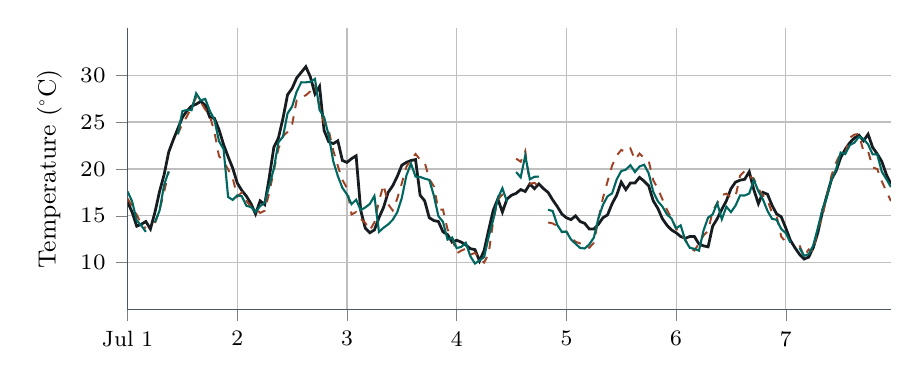
\begin{tikzpicture}\begin{axis}[weather,height=2.03in,xmin=0,xmax=167,ymin=5,ymax=35,xtick={0,24,48,72,96,120,144},xticklabels={Jul 1,2,3,4,5,6,7},ytick={10,15,20,25,30},ylabel={Temperature (\celsius)},ymajorgrids,unbounded coords=jump]
\addplot[ink,line width=1.0pt] coordinates {(0,16.5000) (1,15.4000) (2,13.9000) (3,14.1000) (4,14.4000) (5,13.6000) (6,15.4000) (7,17.6000) (8,19.4000) (9,21.8000) (10,23.1000) (11,24.3000) (12,25.5000) (13,26.2000) (14,26.7000) (15,26.9000) (16,27.2000) (17,26.8000) (18,25.5000) (19,25.4000) (20,24.2000) (21,22.6000) (22,21.3000) (23,20.1000) (24,18.5000) (25,17.7000) (26,17.1000) (27,16.3000) (28,15.2000) (29,16.6000) (30,16.2000) (31,19.1000) (32,22.3000) (33,23.3000) (34,25.4000) (35,27.9000) (36,28.6000) (37,29.7000) (38,30.3000) (39,30.9000) (40,29.8000) (41,28.0000) (42,28.8000) (43,24.1000) (44,22.9000) (45,22.7000) (46,23.0000) (47,20.9000) (48,20.7000) (49,21.1000) (50,21.4000) (51,15.6000) (52,13.7000) (53,13.2000) (54,13.5000) (55,14.8000) (56,15.9000) (57,17.5000) (58,18.2000) (59,19.2000) (60,20.4000) (61,20.7000) (62,20.9000) (63,21.0000) (64,17.2000) (65,16.6000) (66,14.8000) (67,14.5000) (68,14.4000) (69,13.3000) (70,13.0000) (71,12.2000) (72,12.4000) (73,12.2000) (74,11.9000) (75,11.5000) (76,11.4000) (77,10.2000) (78,11.3000) (79,13.5000) (80,15.6000) (81,16.8000) (82,15.4000) (83,16.8000) (84,17.2000) (85,17.4000) (86,17.8000) (87,17.6000) (88,18.4000) (89,17.9000) (90,18.4000) (91,17.9000) (92,17.5000) (93,16.7000) (94,16.0000) (95,15.2000) (96,14.8000) (97,14.6000) (98,15.0000) (99,14.4000) (100,14.2000) (101,13.6000) (102,13.6000) (103,14.1000) (104,14.8000) (105,15.1000) (106,16.3000) (107,17.2000) (108,18.6000) (109,17.8000) (110,18.5000) (111,18.5000) (112,19.1000) (113,18.7000) (114,18.2000) (115,16.6000) (116,15.8000) (117,14.7000) (118,14.0000) (119,13.5000) (120,13.2000) (121,12.8000) (122,12.6000) (123,12.8000) (124,12.8000) (125,12.0000) (126,11.8000) (127,11.7000) (128,13.9000) (129,14.7000) (130,15.7000) (131,16.6000) (132,17.9000) (133,18.6000) (134,18.8000) (135,18.9000) (136,19.7000) (137,17.8000) (138,16.3000) (139,17.5000) (140,17.3000) (141,16.1000) (142,15.2000) (143,14.9000) (144,13.7000) (145,12.4000) (146,11.6000) (147,10.9000) (148,10.4000) (149,10.6000) (150,11.6000) (151,13.2000) (152,15.4000) (153,17.2000) (154,18.9000) (155,19.8000) (156,21.2000) (157,22.1000) (158,22.8000) (159,23.3000) (160,23.6000) (161,23.0000) (162,23.7000) (163,22.3000) (164,21.6000) (165,20.8000) (166,19.4000) (167,18.4000)};
\addplot[rust,dashed,line width=0.70pt] coordinates {(0,16.8514) (1,16.0659) (2,15.1365) (3,14.0940) (4,13.6871) (5,nan) (6,14.2364) (7,15.5992) (8,17.5451) (9,19.7020) (10,nan) (11,23.7285) (12,24.8137) (13,25.6025) (14,26.6358) (15,27.6293) (16,27.1284) (17,26.3326) (18,25.6659) (19,23.9440) (20,21.3737) (21,20.8192) (22,19.9464) (23,19.0263) (24,17.0371) (25,17.5076) (26,16.5819) (27,15.9829) (28,15.8098) (29,15.3168) (30,15.5443) (31,17.4846) (32,19.8350) (33,22.1384) (34,23.4904) (35,23.9503) (36,24.7536) (37,27.3172) (38,27.7063) (39,27.8494) (40,28.2798) (41,29.0147) (42,26.6927) (43,24.8936) (44,24.1272) (45,21.9679) (46,20.3222) (47,18.8330) (48,17.9754) (49,15.1530) (50,15.4064) (51,14.6811) (52,14.2542) (53,13.4643) (54,14.3256) (55,16.5608) (56,18.3303) (57,16.2397) (58,15.5799) (59,16.8425) (60,18.4811) (61,20.2308) (62,20.9956) (63,21.5922) (64,21.0064) (65,20.7096) (66,18.9434) (67,18.1422) (68,15.6698) (69,15.6768) (70,13.5592) (71,12.7217) (72,11.0038) (73,11.2923) (74,11.5033) (75,10.8596) (76,11.0547) (77,10.4458) (78,10.0196) (79,10.9877) (80,14.4676) (81,16.7471) (82,17.2725) (83,17.2141) (84,nan) (85,21.1062) (86,20.7658) (87,21.9086) (88,18.4100) (89,18.5261) (90,18.1092) (91,nan) (92,14.2966) (93,14.1927) (94,13.9151) (95,13.2600) (96,13.3262) (97,12.6694) (98,12.2445) (99,12.0645) (100,11.9336) (101,11.5965) (102,12.1322) (103,14.6334) (104,16.9204) (105,18.6561) (106,20.3592) (107,21.4217) (108,22.0314) (109,21.7778) (110,22.1872) (111,20.9776) (112,21.6389) (113,21.1735) (114,20.8727) (115,18.7955) (116,17.9172) (117,16.7690) (118,15.6515) (119,14.7163) (120,13.6023) (121,13.1285) (122,12.4847) (123,11.5630) (124,11.3065) (125,12.0554) (126,12.9098) (127,13.3979) (128,15.5352) (129,16.3598) (130,17.2247) (131,17.3616) (132,16.9427) (133,17.0690) (134,19.2759) (135,19.7704) (136,19.2188) (137,18.9589) (138,17.8884) (139,17.1657) (140,16.6833) (141,15.2929) (142,14.9821) (143,12.7897) (144,12.2144) (145,12.2645) (146,nan) (147,11.8506) (148,10.6676) (149,11.4238) (150,11.2098) (151,13.6687) (152,14.8814) (153,17.2386) (154,19.3217) (155,20.6889) (156,21.6779) (157,21.6700) (158,23.3391) (159,23.6633) (160,23.7314) (161,21.8431) (162,21.9006) (163,20.1568) (164,19.9959) (165,18.6749) (166,17.6180) (167,16.5723)};
\addplot[teal,line width=.76pt] coordinates {(0,17.5989) (1,16.5446) (2,14.5007) (3,13.9791) (4,13.2929) (5,nan) (6,14.3184) (7,15.5650) (8,18.2966) (9,19.7461) (10,nan) (11,23.6883) (12,26.1579) (13,26.3011) (14,26.2606) (15,28.0641) (16,27.3035) (17,27.4654) (18,26.1835) (19,25.2572) (20,22.9623) (21,22.1195) (22,17.0118) (23,16.7017) (24,17.1926) (25,17.0863) (26,16.0696) (27,15.9390) (28,15.4078) (29,16.0412) (30,16.4021) (31,18.2098) (32,20.0268) (33,22.8369) (34,23.4370) (35,25.9175) (36,26.6532) (37,28.2501) (38,29.2365) (39,29.2308) (40,29.2868) (41,29.5943) (42,26.2855) (43,25.5134) (44,23.5852) (45,20.8162) (46,19.2464) (47,17.9854) (48,17.2873) (49,16.2432) (50,16.7309) (51,15.6097) (52,15.8939) (53,16.2700) (54,17.1199) (55,13.2934) (56,13.7327) (57,14.0892) (58,14.5801) (59,15.3877) (60,16.9165) (61,19.2942) (62,20.5733) (63,19.1806) (64,19.1541) (65,18.9700) (66,18.8327) (67,17.1704) (68,14.9665) (69,14.3679) (70,12.4712) (71,12.6962) (72,11.5603) (73,11.6954) (74,12.1254) (75,10.6837) (76,9.9199) (77,10.2466) (78,10.5979) (79,12.7817) (80,14.6091) (81,16.8779) (82,17.9433) (83,16.5089) (84,nan) (85,19.6740) (86,19.1045) (87,21.4234) (88,18.8948) (89,19.1637) (90,19.1889) (91,nan) (92,15.6559) (93,15.5106) (94,14.0430) (95,13.2994) (96,13.3109) (97,12.4944) (98,12.0276) (99,11.5820) (100,11.5235) (101,11.9563) (102,12.6754) (103,14.7405) (104,16.1788) (105,17.0824) (106,17.3994) (107,18.8855) (108,19.7730) (109,19.9277) (110,20.4022) (111,19.6696) (112,20.2675) (113,20.4480) (114,19.5462) (115,17.5671) (116,16.5566) (117,16.0000) (118,15.1598) (119,14.7057) (120,13.6782) (121,13.9888) (122,12.4031) (123,11.5949) (124,11.4837) (125,11.2968) (126,13.4435) (127,14.8184) (128,15.1593) (129,16.3571) (130,14.6366) (131,15.9766) (132,15.3990) (133,16.0918) (134,17.1797) (135,17.1717) (136,17.3810) (137,18.8235) (138,17.6262) (139,16.7487) (140,15.5233) (141,14.6781) (142,14.5817) (143,13.6044) (144,13.1641) (145,12.1542) (146,nan) (147,11.5823) (148,10.7416) (149,10.9128) (150,11.8439) (151,13.7002) (152,15.6741) (153,17.0593) (154,18.9076) (155,19.9602) (156,21.7537) (157,21.5925) (158,22.5398) (159,22.8016) (160,23.4375) (161,23.1876) (162,22.6195) (163,21.5578) (164,21.5433) (165,19.7075) (166,18.9199) (167,18.0723)};
\end{axis}\end{tikzpicture}
\caption{Six-hour forecasts and observed temperature during 1--7 February (top) and 1--7 July (bottom), 2025. Time is the valid hour in local standard time. Gaps denote unavailable forecasts.}\label{fig:weeks}
\end{figure}


Of 168 valid hours in the February window, 135 had paired forecasts. Airport and regional RMSEs were 2.686 and 2.520\,\celsius. At 09:00 on 4 February, the observed temperature was $-25.6$\,\celsius. The local forecast was $-20.55$ and the regional forecast $-24.25$\,\celsius. At noon on 6 February, the observation was $-9.9$\,\celsius{} and the two forecasts were $-12.01$ and $-15.92$\,\celsius. These hours illustrate both directions of the paired change during the same winter week.


In July, 163 hours had paired forecasts. Observations ranged from 10.2 to 30.9\,\celsius{}, with repeated daytime warming and overnight cooling. RMSE fell from 1.940 to 1.712\,\celsius{} when the five stations were included. Both models captured much of the daily cycle. The full-season comparisons in Section~\ref{seasons} use every eligible hour, including periods outside these two examples.


\subsection{The lead-time error curve}\label{growth}
The five neural-network leads leave large gaps in the error curve. To examine its shape, the project fitted 48 separate regional OLS models, one for each integer lead from 1 to 48 hours. The stored 2025 scores use 8,094--8,102 origins per lead. Intermediate leads have slightly different verification coverage. Persistence uses the same cases as OLS at each lead.

Figure~\ref{fig:growth} places the empirical error curves on the same axes.



\begin{figure}[!htbp]
\centering
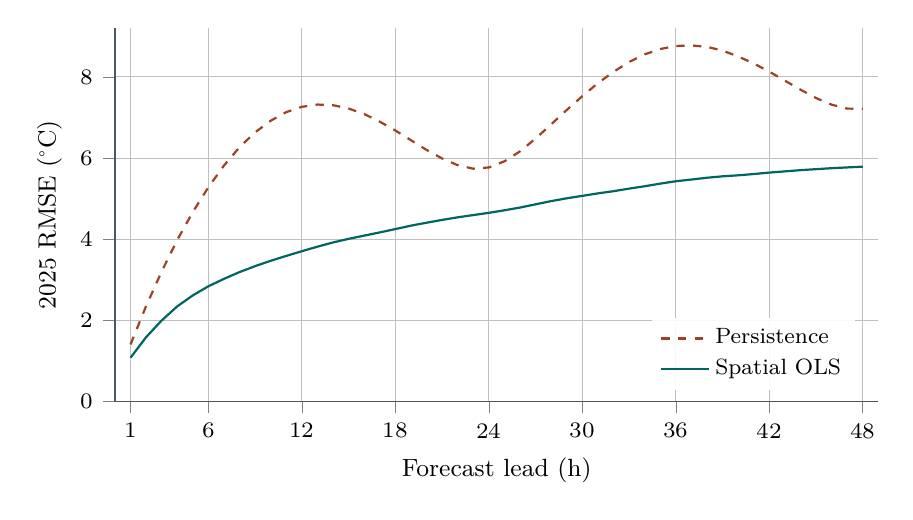
\begin{tikzpicture}\begin{axis}[weather,height=2.49in,xmin=0,xmax=49,ymin=0,ymax=9.2,xtick={1,6,12,18,24,30,36,42,48},ytick={0,2,4,6,8},xlabel={Forecast lead (h)},ylabel={2025 RMSE (\celsius)},ymajorgrids,legend pos=south east]
\addplot[rust,dashed,thick] coordinates {(1,1.4109) (2,2.3555) (3,3.2091) (4,3.9852) (5,4.6734) (6,5.2860) (7,5.8177) (8,6.2716) (9,6.6362) (10,6.9228) (11,7.1341) (12,7.2636) (13,7.3198) (14,7.3042) (15,7.2216) (16,7.0862) (17,6.8981) (18,6.6801) (19,6.4415) (20,6.2017) (21,5.9912) (22,5.8259) (23,5.7397) (24,5.7704) (25,5.9216) (26,6.1675) (27,6.4833) (28,6.8325) (29,7.1859) (30,7.5270) (31,7.8470) (32,8.1257) (33,8.3690) (34,8.5568) (35,8.6872) (36,8.7625) (37,8.7765) (38,8.7411) (39,8.6483) (40,8.5048) (41,8.3315) (42,8.1303) (43,7.9090) (44,7.6880) (45,7.4806) (46,7.3168) (47,7.2202) (48,7.2160)};
\addlegendentry{Persistence}
\addplot[teal,thick] coordinates {(1,1.0838) (2,1.5896) (3,2.0013) (4,2.3482) (5,2.6196) (6,2.8440) (7,3.0260) (8,3.1937) (9,3.3397) (10,3.4716) (11,3.5920) (12,3.7075) (13,3.8190) (14,3.9229) (15,4.0118) (16,4.0909) (17,4.1701) (18,4.2525) (19,4.3365) (20,4.4090) (21,4.4774) (22,4.5416) (23,4.5975) (24,4.6523) (25,4.7151) (26,4.7825) (27,4.8625) (28,4.9409) (29,5.0107) (30,5.0703) (31,5.1318) (32,5.1853) (33,5.2489) (34,5.3069) (35,5.3721) (36,5.4303) (37,5.4725) (38,5.5169) (39,5.5518) (40,5.5767) (41,5.6080) (42,5.6438) (43,5.6735) (44,5.7036) (45,5.7276) (46,5.7522) (47,5.7711) (48,5.7898)};
\addlegendentry{Spatial OLS}
\end{axis}\end{tikzpicture}
\caption{RMSE of persistence and regional ordinary least squares at each integer lead from 1 to 48 hours.}\label{fig:growth}
\end{figure}



Three two-parameter curves were fitted by least squares to the 48 regional OLS RMSEs on the original temperature-error scale, giving each lead equal weight. The last column of Table~\ref{tab:curves} measures the discrepancy between a curve and the 48 measured RMSEs. It is distinct from the error of predicting tomorrow's temperature.


\begin{table}[!htbp]
\centering\small
\caption{Least-squares approximations to the 48 regional OLS RMSEs. Curve RMSE measures discrepancy from the empirical lead-error curve.}\label{tab:curves}
\renewcommand{\arraystretch}{1.11}\begin{tabular*}{.94\linewidth}{@{\extracolsep{\fill}}llrr@{}}\toprule\thead{Form}&\thead{Fitted RMSE at lead $h$}&\thead{$R^2$}&\thead{Curve RMSE (\celsius)}\\\midrule
Power & $1.4784h^{0.3605}$ & 0.99268 & 0.10105 \\
Logarithm & $0.5145+1.3382\log h$ & 0.98728 & 0.13324 \\
Square root & $0.9947+0.7343\sqrt{h}$ & 0.97928 & 0.17002 \\
\bottomrule\end{tabular*}
\end{table}


The power curve follows this particular range most closely. Its exponent below one describes diminishing increments of RMSE. The fits reuse the same 48 empirical scores for estimation and assessment. Neither the ordering nor the exponent establishes a transferable error-growth law.

Raw persistence oscillates. Its RMSE is 7.264\,\celsius{} at 12 hours, 5.770 at 24, 8.763 at 36 and 7.216 at 48. For a daily component $A\cos(2\pi t/24)$, the squared difference between phases $t$ and $t+h$, averaged over a full cycle, equals $2A^2\sin^2(\pi h/24)$. This term vanishes at multiples of 24 and peaks at half days. It illustrates why carrying the current temperature forward can be harder at 12 hours than at 24, even as the weather itself evolves.


\FloatBarrier

\section{Discussion}\label{limits}
For hourly observation-based forecasts at Calgary International Airport, five additional stations improved a matched airport-only MLP at 1, 6, 12 and 24 hours in 2025. The clearest numerical difference occurred at six hours. At this lead, the regional advantage over the airport MLP appeared in each season and after restoring the 378 calm-wind origins. The regional network also beat calendar-adjusted persistence by about 31\% in RMSE. The number of absolute misses of at least 5\,\celsius{} dropped from 496 to 326. At 48 hours, the airport-only and regional errors were close relative to the uncertainty in their difference.

\paragraph{Scope of inference.}
One target station and one test year supply every headline score. Serially dependent hourly errors do not furnish 8,102 independent replications of a year or location. The case definition also favours origins with a complete local history and all five verifying temperatures. Zero-wind sensitivity measures one known selection effect. Missing local temperature or humidity, prolonged outages and additional stations could produce different performance.

Historical records can include revisions. The feature timestamp specifies the observation hour, while a live system also needs to know when that observation became available. A station that reports after the forecast issue time may contribute to a retrospective vector before it could contribute in service. A live evaluation would preserve as-issued station snapshots, simulate release delays and score on a continuously logged issuance schedule. The measured baselines here are station-based. The project has no matched operational numerical weather prediction forecast for estimating relative skill against a weather service.

\paragraph{Model interpretation.}
The matched MLP comparison estimates the effect of adding regional inputs under one fitting procedure. Input width changes model capacity. Independently fitted OLS ablations isolate a station's contribution within that class of models. None of the tests establishes a physical transport mechanism. The temperature-band results condition on the future observation, so they can diagnose error patterns but cannot be used directly to select a model at forecast time.

The bootstraps condition on the fitted models and the 2025 archive. The calendar baselines, tail analyses, week plots and gradient groups were added after examining the project. For a follow-up experiment, the cutoff for each training window, benchmark list and primary score could be fixed in advance, with forecasts saved before each new season. Rolling-origin evaluations across several years would show whether the two-day sign change and the concentration of six-hour gains in winter recur. Matched as-issued numerical forecasts would make an operational comparison possible.


\section{Conclusion}
For the 2025 YYC verification sample, additional surface stations contributed the most incremental skill at six hours. A decrease in the frequency of large misses and a concentration of squared-error savings in winter account for much of the aggregate improvement. The experiment gives weaker evidence for an advantage at longer leads, and a future evaluation across several years would be needed to quantify year-to-year variation in these estimates.
\appendix


\section{Inference from the fitted networks}\label{inference}
The replication package includes a desktop application for inference from manually entered observations. From the project directory, launch \code{python forecast\_gui.py}. The initial form contains the labelled historical case used in Table~\ref{tab:example}. Select a model and one or more lead times, edit the station readings, and select \emph{Calculate forecast}. The program displays temperatures in \celsius{} and the corresponding local valid times. The issue date and hour generate the cyclic calendar coordinates, and the airport wind direction is converted from degrees to its sine and cosine. For sequence models the interface accepts station histories and a checkpoint seed.

The software calls the same prediction routine as the command-line interface and applies the preprocessing quantities learned from training data. A blank optional regional reading is median-imputed. A blank sequence reading also sets its observation mask to zero. A physical zero remains an observed value. The airport and regional MLPs use 34 and 67 engineered features, respectively. The joint models take 24 hourly vectors of 24 physical measurements and four calendar coordinates.
\paragraph{A worked forecast.}
The example uses archived observations timestamped 00:00 local standard time on 1 January 2025. YYC's temperature was $-12.6$\,\celsius{}, its dew point $-14.5$\,\celsius{}, relative humidity 85\%, and wind speed 13 km/h. The most recent Bow Valley reading was $-11.5$\,\celsius. All other predictors are supplied in the example file.


\begin{table}[!htbp]
\centering\small
\caption{Predicted and subsequently observed temperatures for the origin 1 January 2025, 00:00 LST.}\label{tab:example}
\renewcommand{\arraystretch}{1.10}\begin{tabular*}{.94\linewidth}{@{\extracolsep{\fill}}lrrr@{}}\toprule\thead{Lead}&\thead{Airport MLP (\celsius)}&\thead{Regional MLP (\celsius)}&\thead{Later observed (\celsius)}\\\midrule
1 h & −13.043 & −12.725 & −13.6 \\
6 h & −14.402 & −14.028 & −13.7 \\
12 h & −13.809 & −12.813 & −15.5 \\
24 h & −15.345 & −13.637 & −14.9 \\
48 h & −12.278 & −10.286 & −17.5 \\
\bottomrule\end{tabular*}
\end{table}


To see one feature's numerical influence, change only the current Bow Valley temperature from $-11.5$ to $-10.5$\,\celsius{}. The regional six-hour output moves from $-14.028$ to $-13.988$\,\celsius. This deliberately holds correlated readings fixed and measures the response of the fitted function.


\section{Computational reproducibility}\label{reproduce}
From the extracted project root, use Python 3.12 with NumPy and pandas for the verification and diagnostic commands. The prediction command needs NumPy alone. Run the commands below in an activated environment. The README includes equivalent PowerShell setup and the optional dependencies for refitting.
\begin{codeblock}
python verify_results.py
python -m report.analyze_diagnostics
python -m unittest discover -s tests -v
python predict.py --input examples/spatial.json --lead 6
\end{codeblock}
The first command checks matches between forecast origins, targets and archived station temperatures, recomputes reported scores and replays the ten matched MLP weight sets. The second regenerates the expanded analyses. Regression tests compare predictions from all 21 saved neural checkpoints against archived cases at all five leads. The last command returns $-14.028$\,\celsius{} for the bundled example.

Table~\ref{tab:files} identifies the associated replication materials.



\begin{table}[!htbp]
\centering\small
\caption{Locations of the data definitions, evaluation outputs and inference software in the replication package.}\label{tab:files}
\renewcommand{\arraystretch}{1.14}\begin{tabularx}{.98\linewidth}{@{}p{1.46in}X@{}}\toprule\thead{Evidence}&\thead{Location in the project}\\\midrule
Regional feature definitions & \code{spatial\_extension/data/processed/spatial\_feature\_manifest.csv}\\
Primary uncertainty and calm sensitivity & \code{results/verification/}\\
Model comparisons, OLS ablation and 48-lead curves & \code{architecture\_extension/results/}\\
New matched analyses and time series & \code{report/results/} and \code{report/analyze\_diagnostics.py}\\
Inference applications & \code{forecast\_gui.py}, \code{predict.py}, \code{inference/forecast\_weights.npz}, \code{examples/}\\\bottomrule\end{tabularx}
\end{table}


The separate \LaTeX{} file embeds all plot coordinates and table values. Compile it twice with XeLaTeX to resolve page references. The supplied project also includes the resulting PDF.


\FloatBarrier
\begin{thebibliography}{9}\setlength{\itemsep}{2pt}
\bibitem{eccc} Environment and Climate Change Canada. \href{https://climate.weather.gc.ca/}{Historical Climate Data} and \href{https://climate.weather.gc.ca/glossary_e.html}{glossary of climate terms}. Station identifiers are listed in Table~\ref{tab:stations}.
\bibitem{murphy} A. H. Murphy (1988). \href{https://journals.ametsoc.org/view/journals/mwre/116/12/1520-0493_1988_116_2417_ssbotm_2_0_co_2.xml}{Skill Scores Based on the Mean Square Error and Their Relationships to the Correlation Coefficient}. \emph{Monthly Weather Review} 116, 2417--2424.
\bibitem{politis} D. N. Politis and J. P. Romano (1992). \href{https://mathweb.ucsd.edu/~politis/DPpublication.html}{A Circular Block-Resampling Procedure for Stationary Data}. In \emph{Exploring the Limits of Bootstrap}, Wiley, 263--270.
\bibitem{lightgbm} G. Ke et al.\ (2017). \href{https://proceedings.nips.cc/paper/2017/hash/6449f44a102fde848669bdd9eb6b76fa-Abstract.html}{LightGBM: A Highly Efficient Gradient Boosting Decision Tree}. \emph{Advances in Neural Information Processing Systems} 30.
\bibitem{tcn} S. Bai, J. Z. Kolter and V. Koltun (2018). \href{https://arxiv.org/abs/1803.01271}{An Empirical Evaluation of Generic Convolutional and Recurrent Networks for Sequence Modeling}. arXiv:1803.01271.
\end{thebibliography}
\end{document}
